% Ubah kalimat sesuai dengan judul dari bab ini
\chapter{PENGUJIAN DAN EVALUASI}
\vspace{4ex}

% Pengaturan ukuran indentasi
\setlength{\parindent}{7ex}

% Ubah konten-konten berikut sesuai dengan yang ingin diisi pada bab ini

\section{Lingkungan Pengujian}
\vspace{1ex}

Pengujian yang kami lakukan menggunakan VPS (\emph{Virtual Private Server}) sebagai media yang digunakan untuk menjalankan sistem yang kami buat secara online.
Pada VPS tersebut, kami mempersiapkan beberapa hal yang diperlukan agar sistem bisa berjalan dengan semestinya.
Persiapan yang dijelaskan tersebut terdiri dari instalasi library dan framework yang dibutuhkan, instalasi dan konfigurasi database, konfigurasi DNS (\emph{Domain Name System}), konfigurasi service, dan lain sebagainya.
\vspace{0.5ex}

Setelah server sudah siap untuk digunakan, kami kemudian mempersiapkan dua jenis perangkat untuk menguji fungsionalitas dari sistem yang telah kami buat.
Pengujian tersebut akan dilakukan menggunakan sebuah perangkat desktop yang mengakses website secara langsung dan sebuah perangkat mobile yang mengakses server tersebut melalui PWA.
\vspace{0.5ex}

\section{Skenario Pengujian}
\vspace{1ex}

Pengujian yang kami lakukan akan mencakup keseluruhan aspek yang dimiliki oleh sistem yang telah kami buat.
Detail dari aspek-aspek tersebut adalah sebagai berikut:
\vspace{0.5ex}

\begin{enumerate}[nolistsep]

  \item Menguji sistem login dan pendaftaran akun baru.
  \vspace{0.5ex}

  \item Menguji penambahan, pengubahan, dan penghapusan data.
  \vspace{0.5ex}

  \item Menguji PWA pada perangkat mobile.
  \vspace{0.5ex}

  \item Menguji pengunduhan data dalam bentuk \emph{spreadsheet}.
  \vspace{0.5ex}

\end{enumerate}
\vspace{0.5ex}

\newpage

\section{Tahapan Pengujian dan Evaluasi}
\vspace{1ex}

Pada bagian ini, kami akan membahas tahapan-tahapan pengujian yang kami lakukan beserta evaluasinya dengan memperhatikan aspek-aspek yang telah dijelaskan sebelumnya.
Untuk mempersingkat cakupan bahasan pada buku ini, pengujian tidak akan dilakukan pada keseluruhan fitur yang ada pada sistem yang kami buat, namun cukup beberapa fitur yang secara umum sudah mewakili aspek-aspek tersebut.
\vspace{0.5ex}

\subsection{Menguji Sistem Login dan Pendaftaran Akun Baru}
\vspace{1ex}

Pada pengujian ini, kami mencoba membuat akun baru pada sistem sesuai dengan yang ada pada gambar \ref{fig:mendaftarAkun}.
Akun baru yang dibuat ini nantinya akan digunakan oleh pihak karyawan yang ditugaskan untuk melakukan pencatatan administrasi loading barang agar bisa mengakses fungsionalitas pada sistem yang dibuat.
\vspace{0.5ex}

\begin{figure} [ht!] \centering
  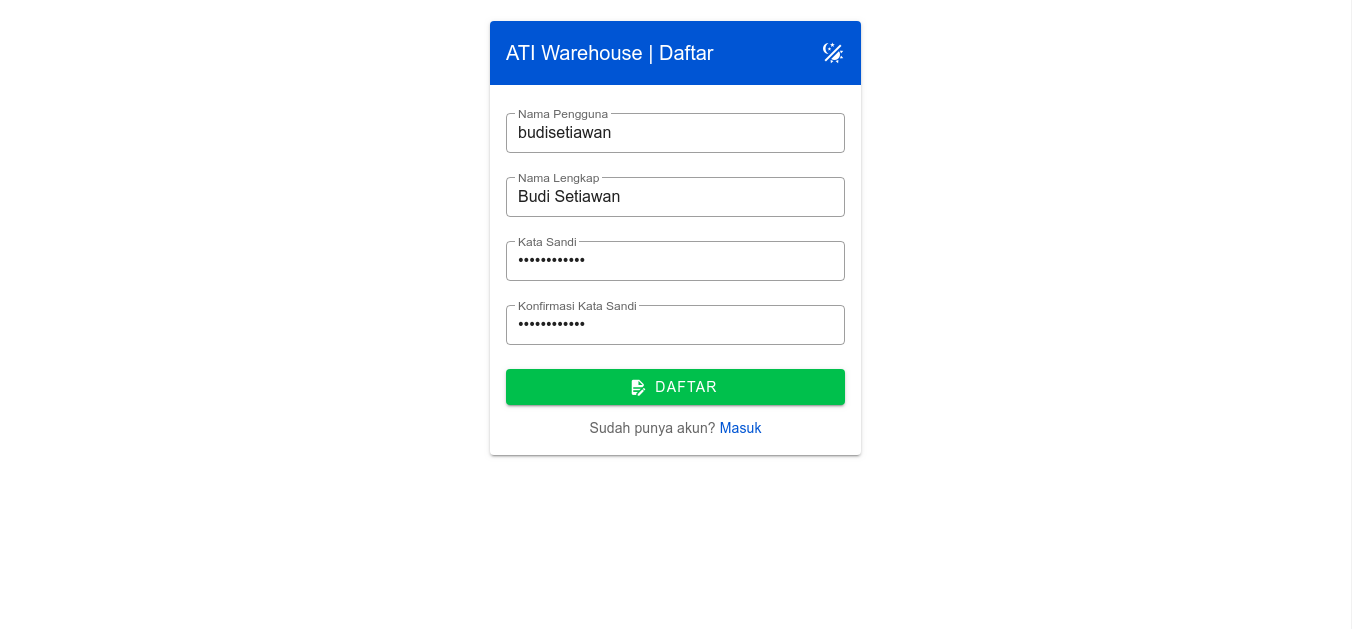
\includegraphics[width=0.95\textwidth]{gambar/mendaftar-akun.png}
  \caption{Tampilan Halaman Pendaftaran Akun Baru}
  \label{fig:mendaftarAkun}
\end{figure}

Pada sistem yang kami buat, sebelum bisa login, akun baru harus diverifikasi terlebih dahulu oleh admin untuk menghindari akses dari akun yang tidak diinginkan.
Verifikasi sendiri bisa dilakukan pada halaman daftar pengguna menggunakan akun admin seperti yang terlihat pada gambar \ref{fig:daftarPengguna}.
\vspace{0.5ex}

\begin{figure} [ht!] \centering
  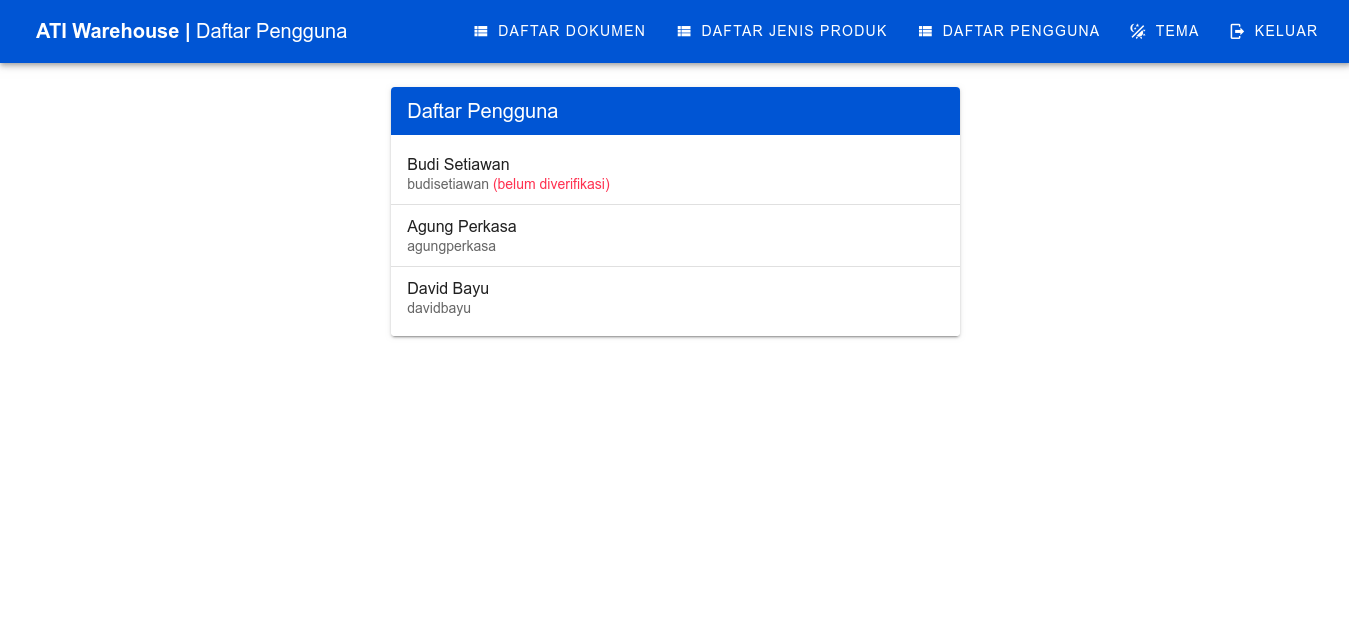
\includegraphics[width=0.95\textwidth]{gambar/daftar-pengguna.png}
  \caption{Tampilan Halaman Daftar Pengguna}
  \label{fig:daftarPengguna}
\end{figure}

\newpage

Pengujian kemudian dilanjutkan dengan melakukan login menggunakan akun yang sudah diverifikasi sebelumnya seperti yang terlihat pada gambar \ref{fig:loginAkun}.
Setelah login berhasil, tampilan akan berpindah ke halaman utama yang berisi data dari keseluruhan administrasi loading barang.
\vspace{0.5ex}

\begin{figure} [ht!] \centering
  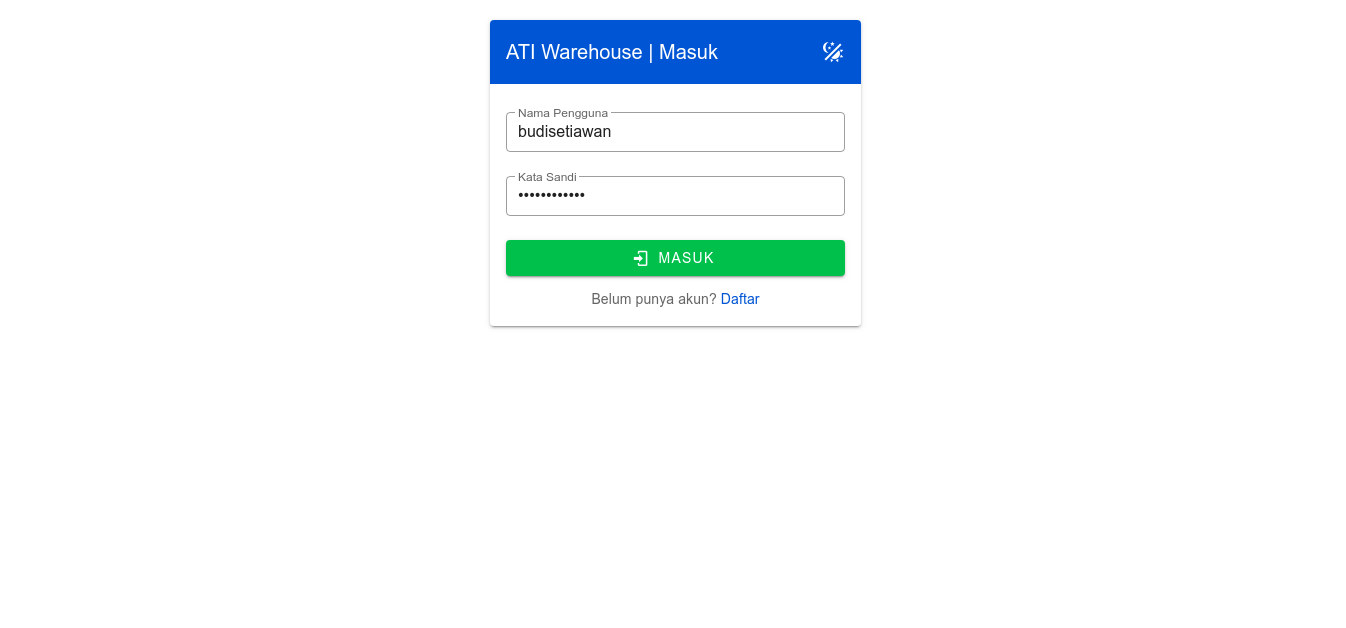
\includegraphics[width=0.95\textwidth]{gambar/login-akun.png}
  \caption{Tampilan Halaman Login Akun}
  \label{fig:loginAkun}
\end{figure}

Dari pengujian yang telah dilakukan tersebut dapat disimpulkan bahwa sistem yang telah kami buat bisa digunakan untuk melakukan login serta registrasi untuk pembuatan akun baru.
Dengan ini, nantinya pengguna yang membutuhkan akses terhadap data administrasi loading barang bisa membuat akun baru yang kemudian dapat diverifikasi oleh admin agar bisa mengakses data tersebut.
\vspace{0.5ex}

\subsection{Menguji Penambahan, Pengubahan, dan Penghapusan Data}
\vspace{1ex}

Pada pengujian ini, kami mencoba melakukan penambahan data palet sesuai dengan tabel \ref{tb:dataPalet}.
Penambahan data palet ini dilakukan pada halaman detail dokumen dengan mengklik tombol tambah data palet.
Setelah tombol diklik, maka akan muncul jendela baru seperti yang terlihat pada gambar \ref{fig:tambahPalet}.
\vspace{0.5ex}

\begin{longtable}{|l|l|l|l|l|}
  \caption{Data Palet}
  \label{tb:dataPalet}\\
  \hline
  \rowcolor[HTML]{C0C0C0}
  \textbf{Mulai} & \textbf{Selesai} & \textbf{Palet} & \textbf{Basket} & \textbf{Jumlah Layer} \\ \hline
  13:03 & 13:34 & 1 & 1, 2, 3 & 18 \\ \hline
  13:34 & 13:49 & 2 & 3, 4, 5 & 18 \\ \hline
  13:49 & 14:05 & 3 & 5, 6, 7 & 18 \\ \hline
  14:05 & 14:26 & 4 & 7, 8, 9 & 18 \\ \hline
  14:26 & 14:35 & 5 & 9, 10, 11, 12 & 18 \\ \hline
  14:35 & 14:50 & 6 & 12, 13, 14 & 18 \\ \hline
\end{longtable}

\begin{figure} [ht!] \centering
  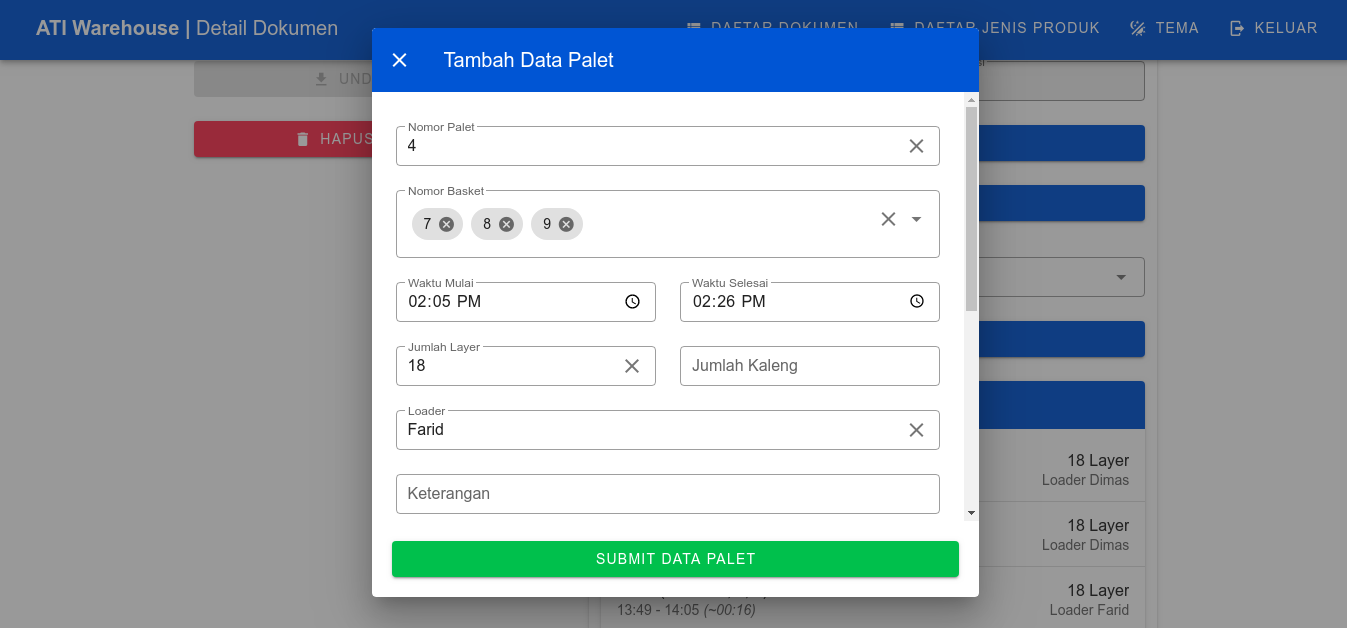
\includegraphics[width=0.95\textwidth]{gambar/tambah-palet.png}
  \caption{Tampilan Jendela Tambah Data Palet}
  \label{fig:tambahPalet}
\end{figure}

Pengujian kemudian dilanjutkan dengan mengubah jumlah layer pada palet nomor 5 menjadi sebanyak 15.
Pengubahan data palet ini dilakukan pada halaman detail palet seperti yang terlihat pada gambar \ref{fig:ubahPalet}.
\vspace{0.5ex}

\begin{figure} [ht!] \centering
  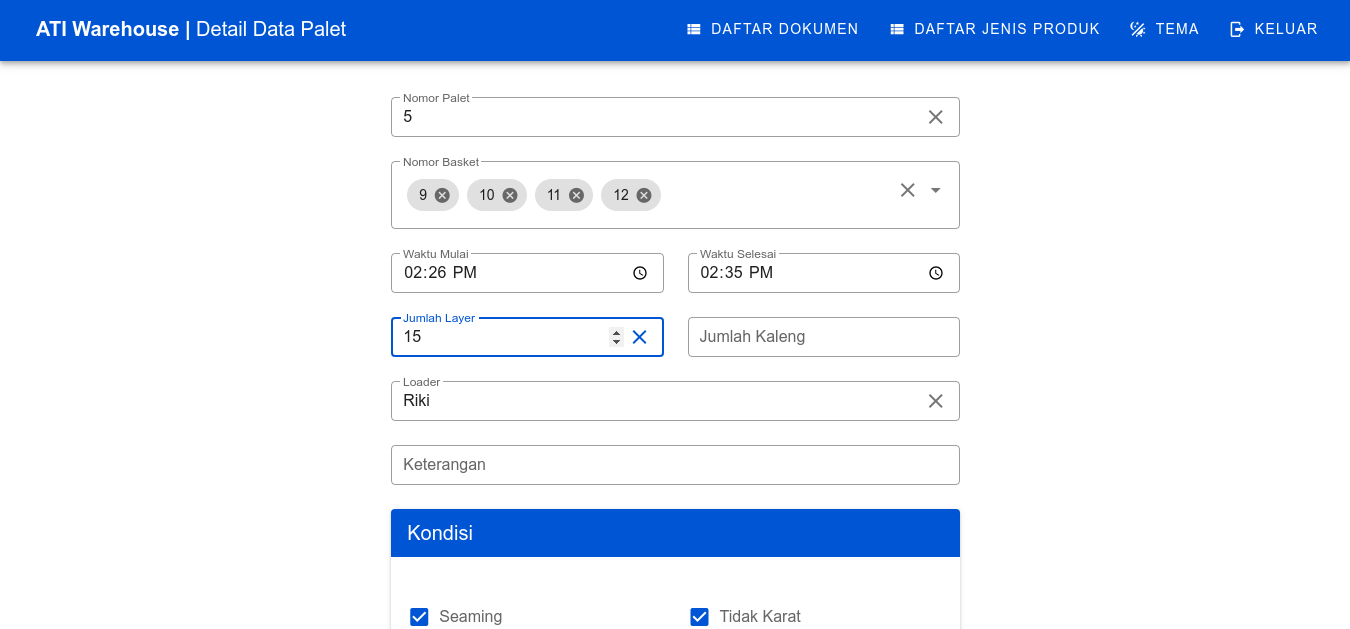
\includegraphics[width=0.95\textwidth]{gambar/ubah-palet.png}
  \caption{Tampilan Halaman Detail Palet}
  \label{fig:ubahPalet}
\end{figure}

Terakhir, pengujian kemudian dilanjutkan dengan menghapus data pada palet nomor 6.
Penghapusan data palet ini juga dilakukan pada halaman detail palet seperti pada percobaan sebelumnya dengan menekan tombol hapus data palet.
Hasil akhir dari percobaan ini adalah kumpulan data palet seperti yang terlihat pada gambar \ref{fig:daftarPalet}.
\vspace{0.5ex}

\begin{figure} [ht!] \centering
  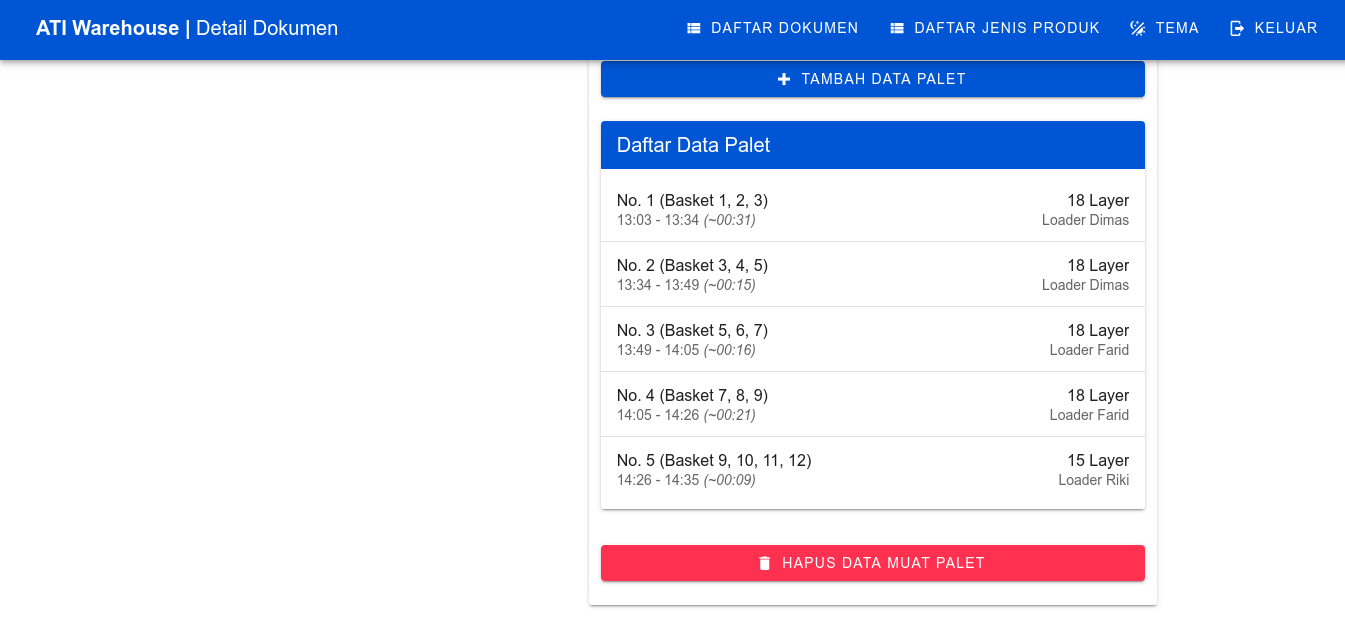
\includegraphics[width=0.95\textwidth]{gambar/daftar-palet.png}
  \caption{Tampilan Daftar Palet}
  \label{fig:daftarPalet}
\end{figure}

Dari pengujian yang telah dilakukan tersebut, dapat disimpulkan bahwa sistem yang telah kami buat bisa digunakan untuk melakukan penambahan, pengubahan, serta penghapusan data sesuai dengan struktur data yang telah ditentukan oleh sistem.
Dengan ini, nantinya sistem yang kami buat bisa digunakan untuk menampung serta menampilkan data administrasi loading barang, menggantikan metode sebelumnya yang masih berbasis kertas.
\vspace{0.5ex}

\subsection{Menguji PWA Pada Perangkat Mobile}
\vspace{1ex}

Pada pengujian kali ini, kami mencoba menguji penggunaan PWA dari system yang telah kami buat pada perangkat mobile.
Pemasangan PWA sendiri bisa dilakukan dengan cara mengakses website dari sistem yang telah kami buat pada perangkat mobile.
Pada website yang mendukung fitur PWA, umumnya browser akan menawarkan penambahan website tersebut sebagai aplikasi pada perangkat mobile seperti yang terlihat pada gambar \ref{fig:pasangPwa}.
\vspace{0.5ex}

\begin{figure} [ht!] \centering
  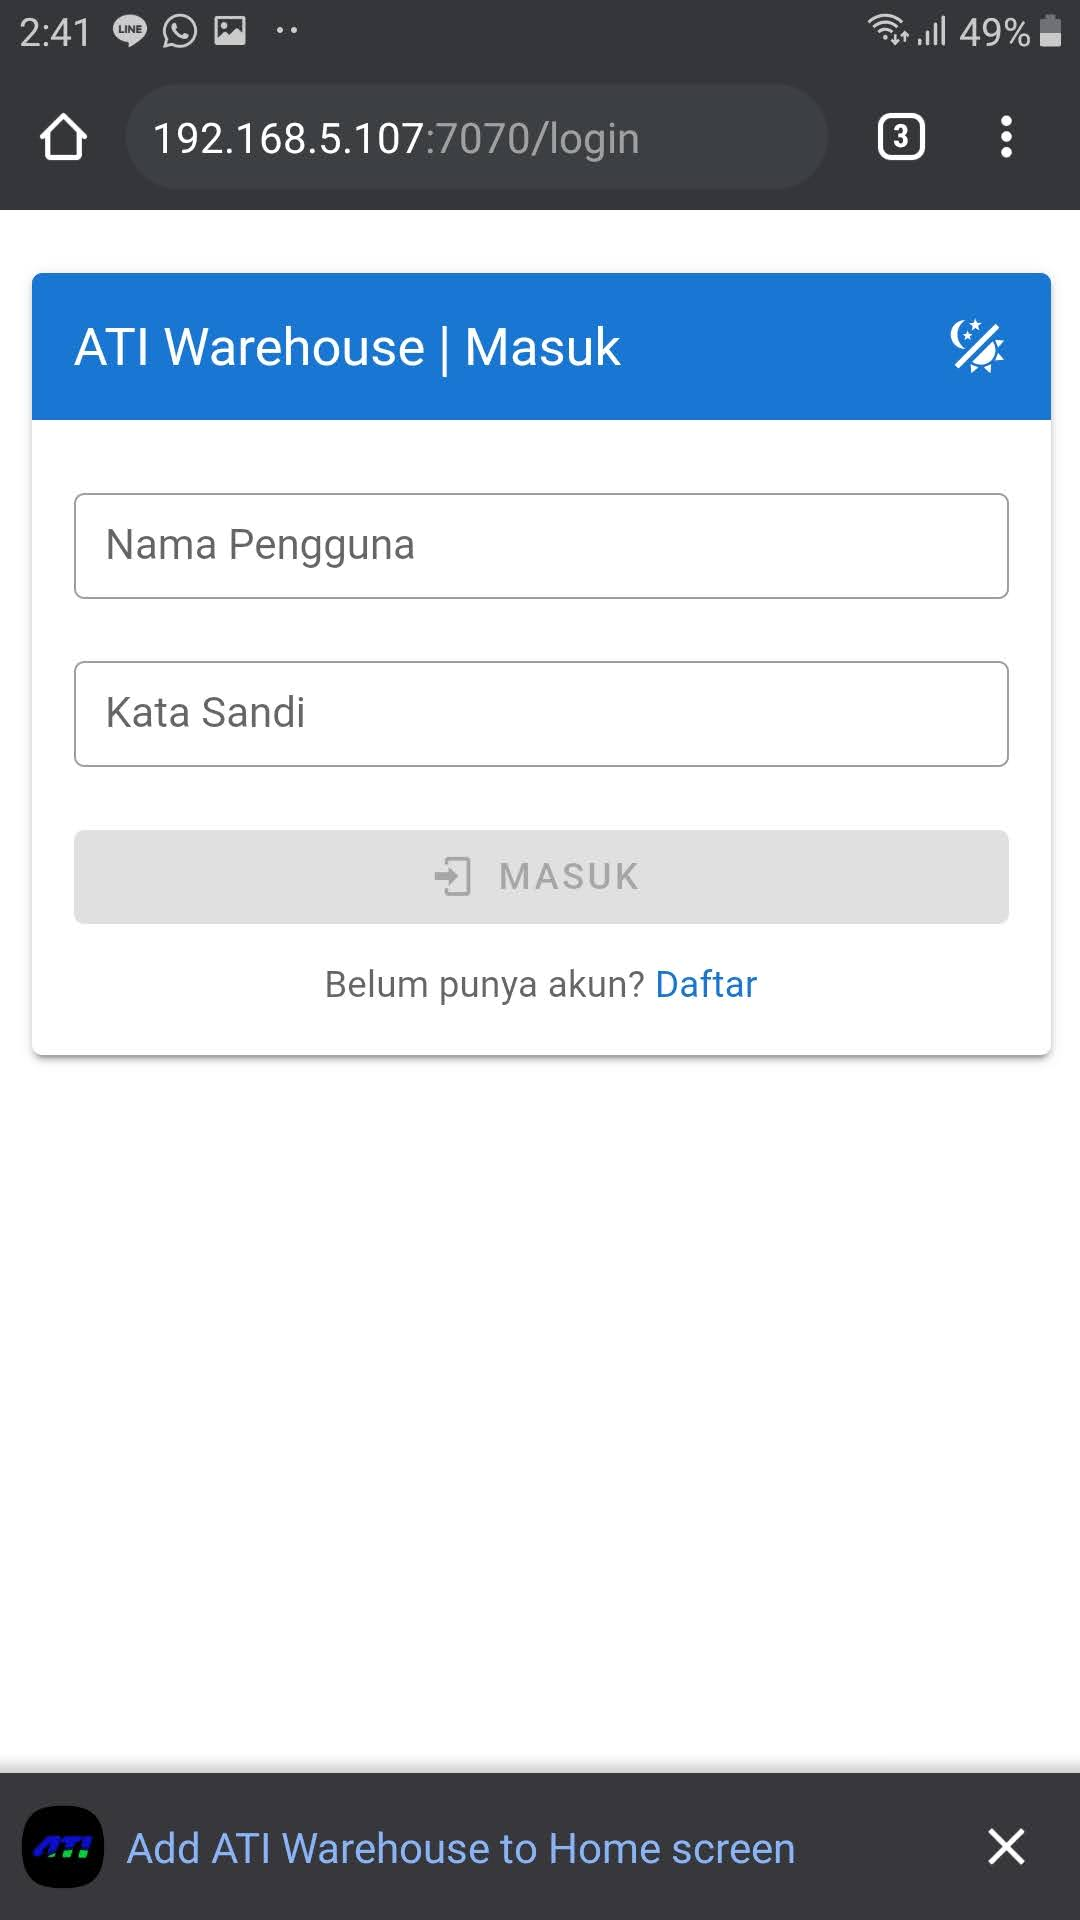
\includegraphics[width=0.45\textwidth]{gambar/pasang-pwa.jpg}
  \caption{Tawaran Penambahan Website Sebagai PWA}
  \label{fig:pasangPwa}
\end{figure}

Setelah terpasang, sistem yang kami buat akan tampak pada daftar aplikasi yang ada di perangkat mobile selayaknya aplikasi pada umumnya.
Selain itu, PWA yang telah kami pasang nantinya bisa berfungsi selayaknya sistem yang juga terpasang pada website seperti terlihat pada gambar \ref{fig:tampilanPwa}.
Dengan ini, alih-alih mengakses website untuk menggunakan sistem yang telah kami buat,  pengguna juga bisa memasang langsung sistem tersebut pada perangkat mereka, sehingga mempermudah akses dari sistem administrasi loading barang ini.
\vspace{0.5ex}

\begin{figure} [ht!] \centering
  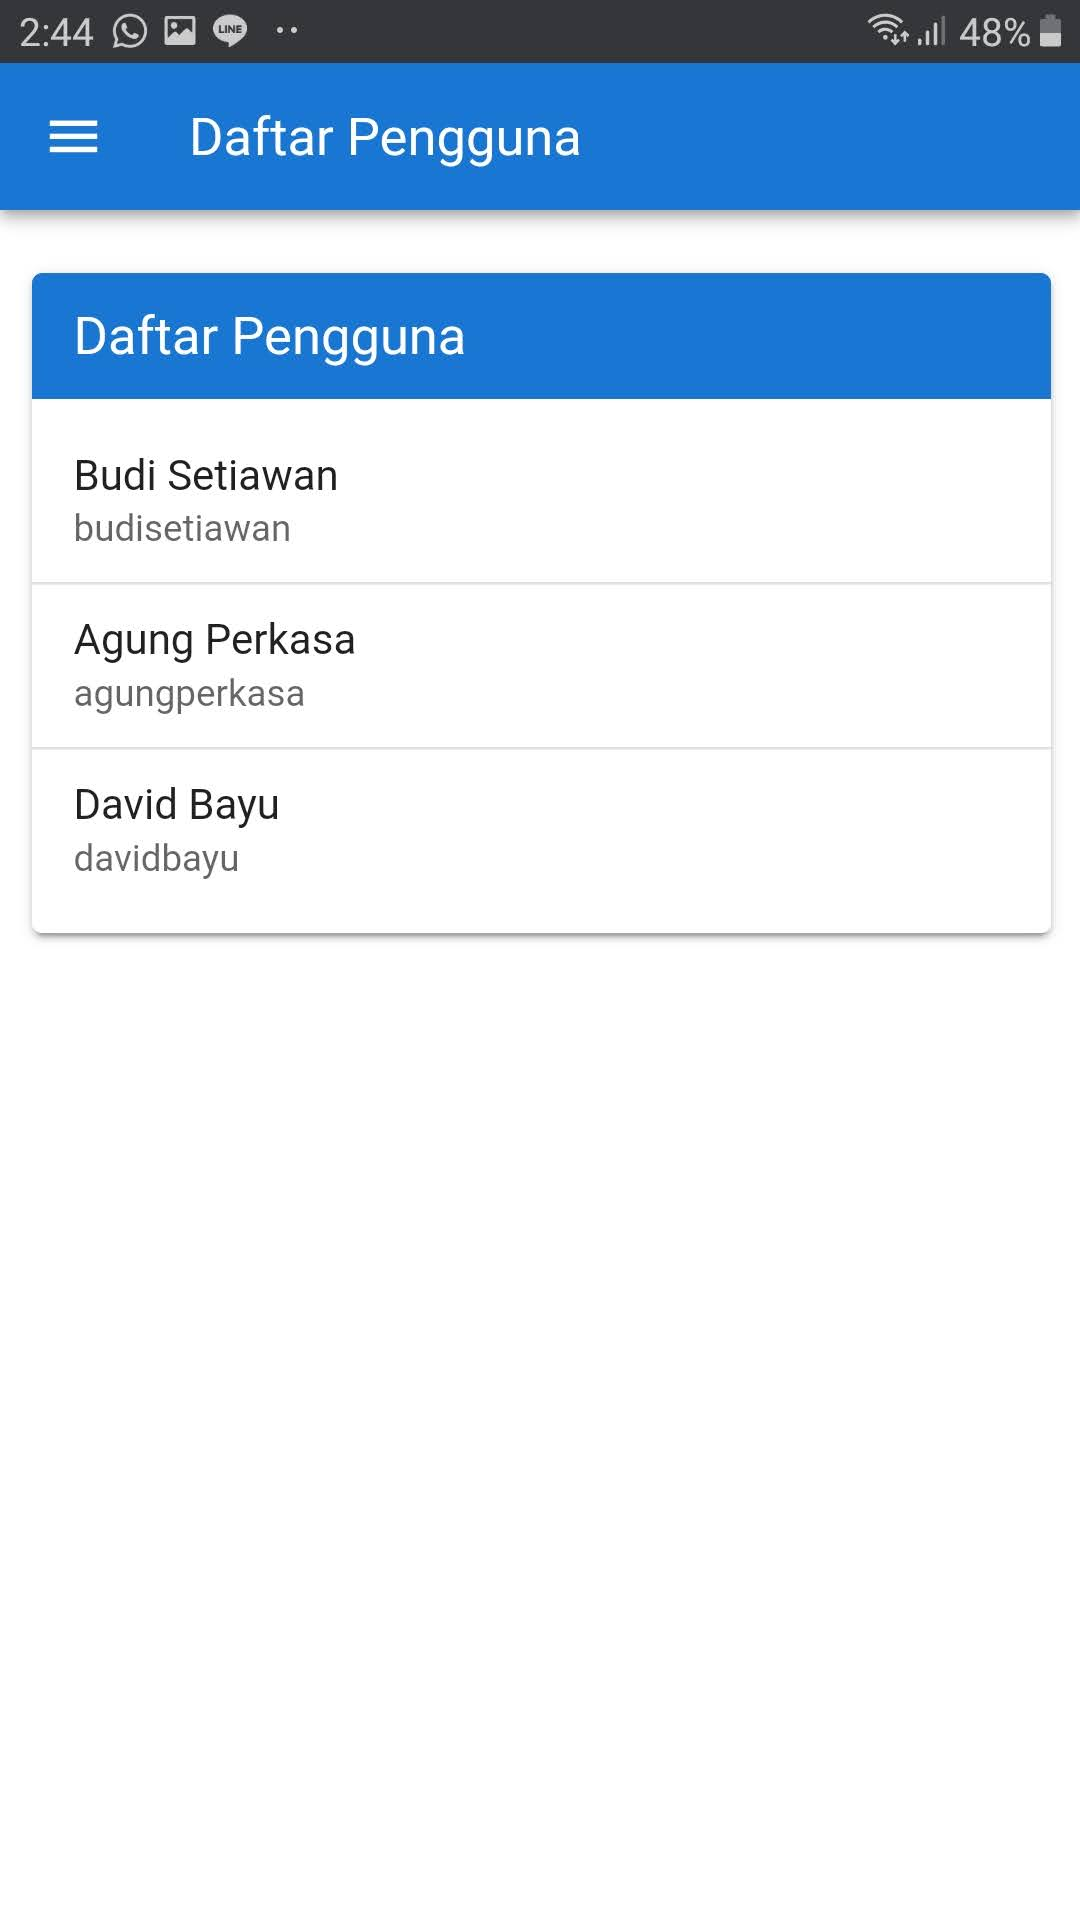
\includegraphics[width=0.45\textwidth]{gambar/tampilan-pwa-1.jpg}
  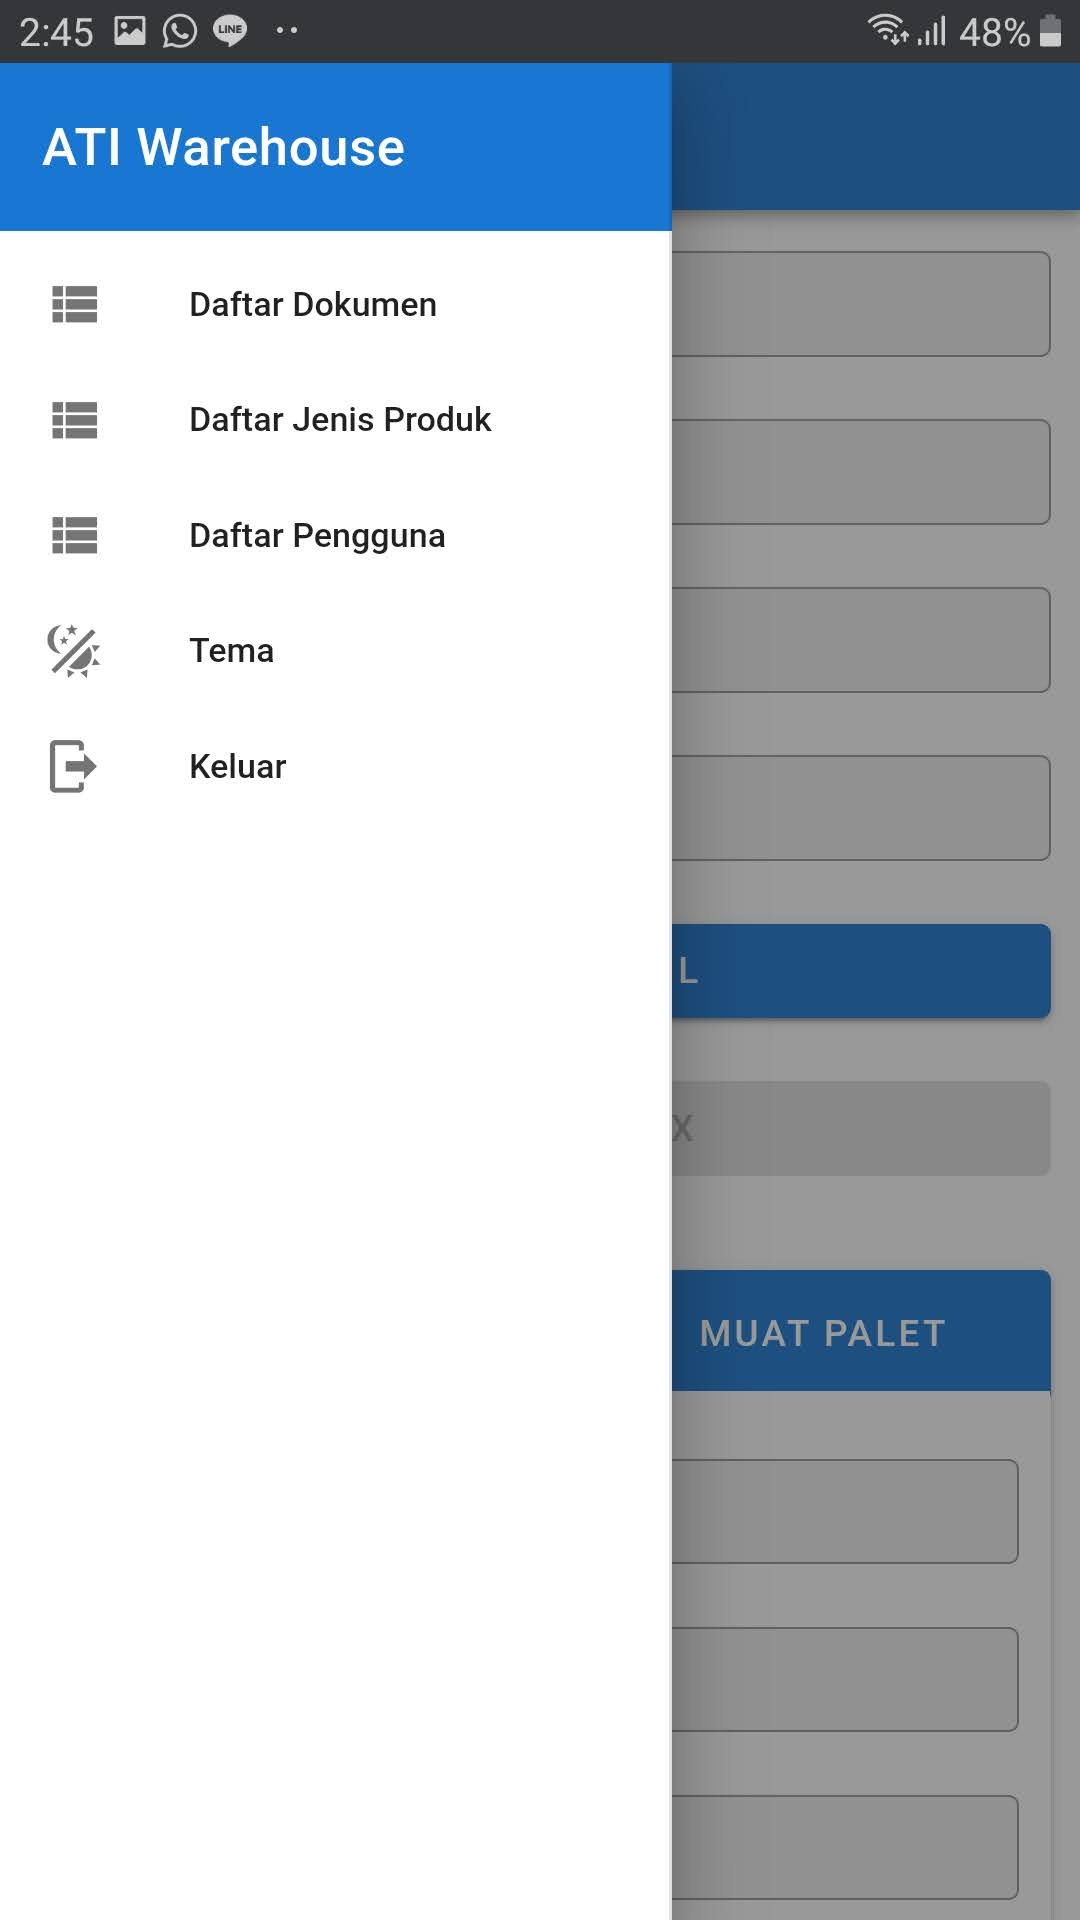
\includegraphics[width=0.45\textwidth]{gambar/tampilan-pwa-2.jpg}
  \caption{Tampilan PWA Pada Perangkat Mobile}
  \label{fig:tampilanPwa}
\end{figure}

\subsection{Menguji Pengunduhan Data Dalam Bentuk \emph{Spreadsheet}}
\vspace{1ex}

Pada pengujian terakhir ini, kami mencoba menguji pengunduhan data dalam bentuk \emph{spreadsheet} yang ada pada sistem yang telah kami buat.
Pengunduhan data dalam bentuk \emph{spreadsheet} tersebut bisa dilakukan pada halaman detail dokumen dengan menekan tombol unduh xlsx.
Hasil dari pengunduhan tersebut adalah file dalam bentuk \emph{spreadsheet} yang jika dibuka akan berisi data seperti pada gambar \ref{fig:isiSpreadsheet}.
\vspace{0.5ex}

\newpage

\begin{figure} [ht!] \centering
  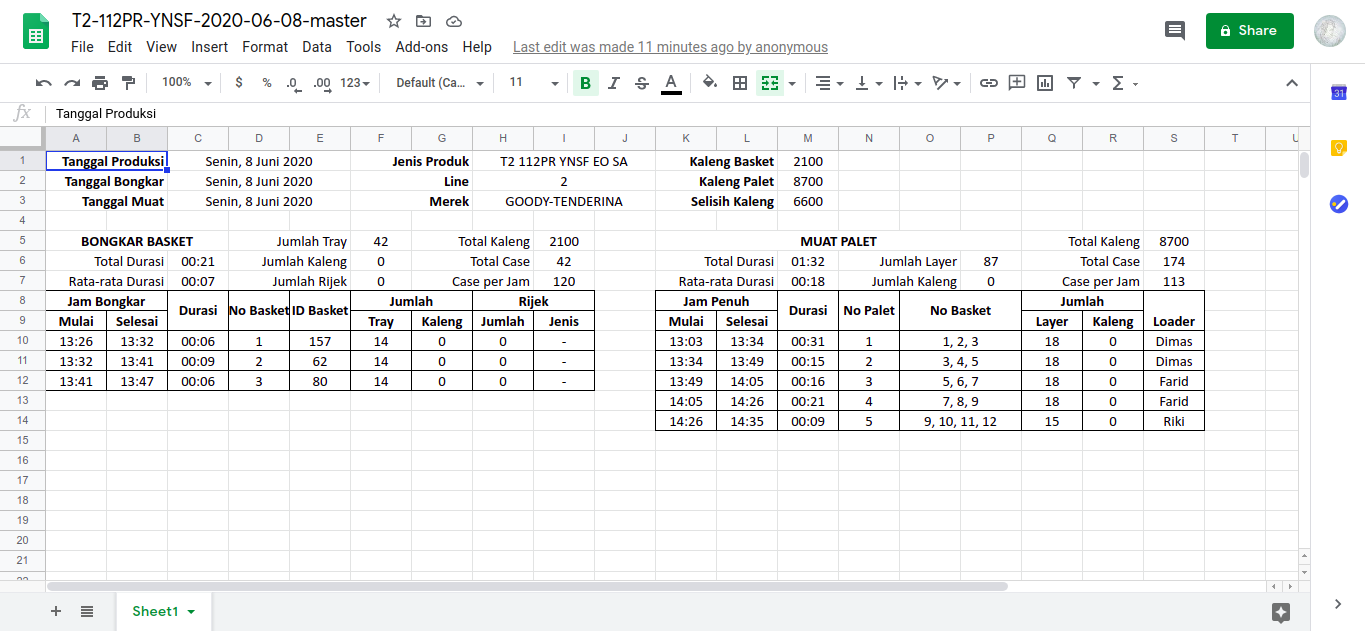
\includegraphics[width=0.95\textwidth]{gambar/isi-spreadsheet.png}
  \caption{Isi Dari File Spreadsheet yang Diunduh}
  \label{fig:isiSpreadsheet}
\end{figure}

Dari pengujian yang telah dilakukan tersebut, dapat disimpulkan bahwa data yang ada pada sistem yang kami buat bisa diunduh menjadi file \emph{spreadsheet} yang nantinya bisa dicetak.
Dengan ini, walaupun sistem yang kami buat mampu digunakan untuk menggantikan metode sebelumnya yang berbasis kertas, sistem yang kami buat masih bisa menghasilkan laporan yang sama dalam bentuk cetak seperti metode yang ada sebelumnya.
\vspace{0.5ex}
